\chapter{Theoretische Grundlagen}\label{theorie}
%---------------------------------------------------------------------------------------------------------------------------------------------------------------------------------
\section{Der Cubesat Designstandard}%-------------------------------------------------------------------------------------------------------------------------------------------
	\subsection{Historische Entwicklung}
	\hfill\emph{(Valentina Dietrich)}\\
				\begin{figure}[H]
				\centering
					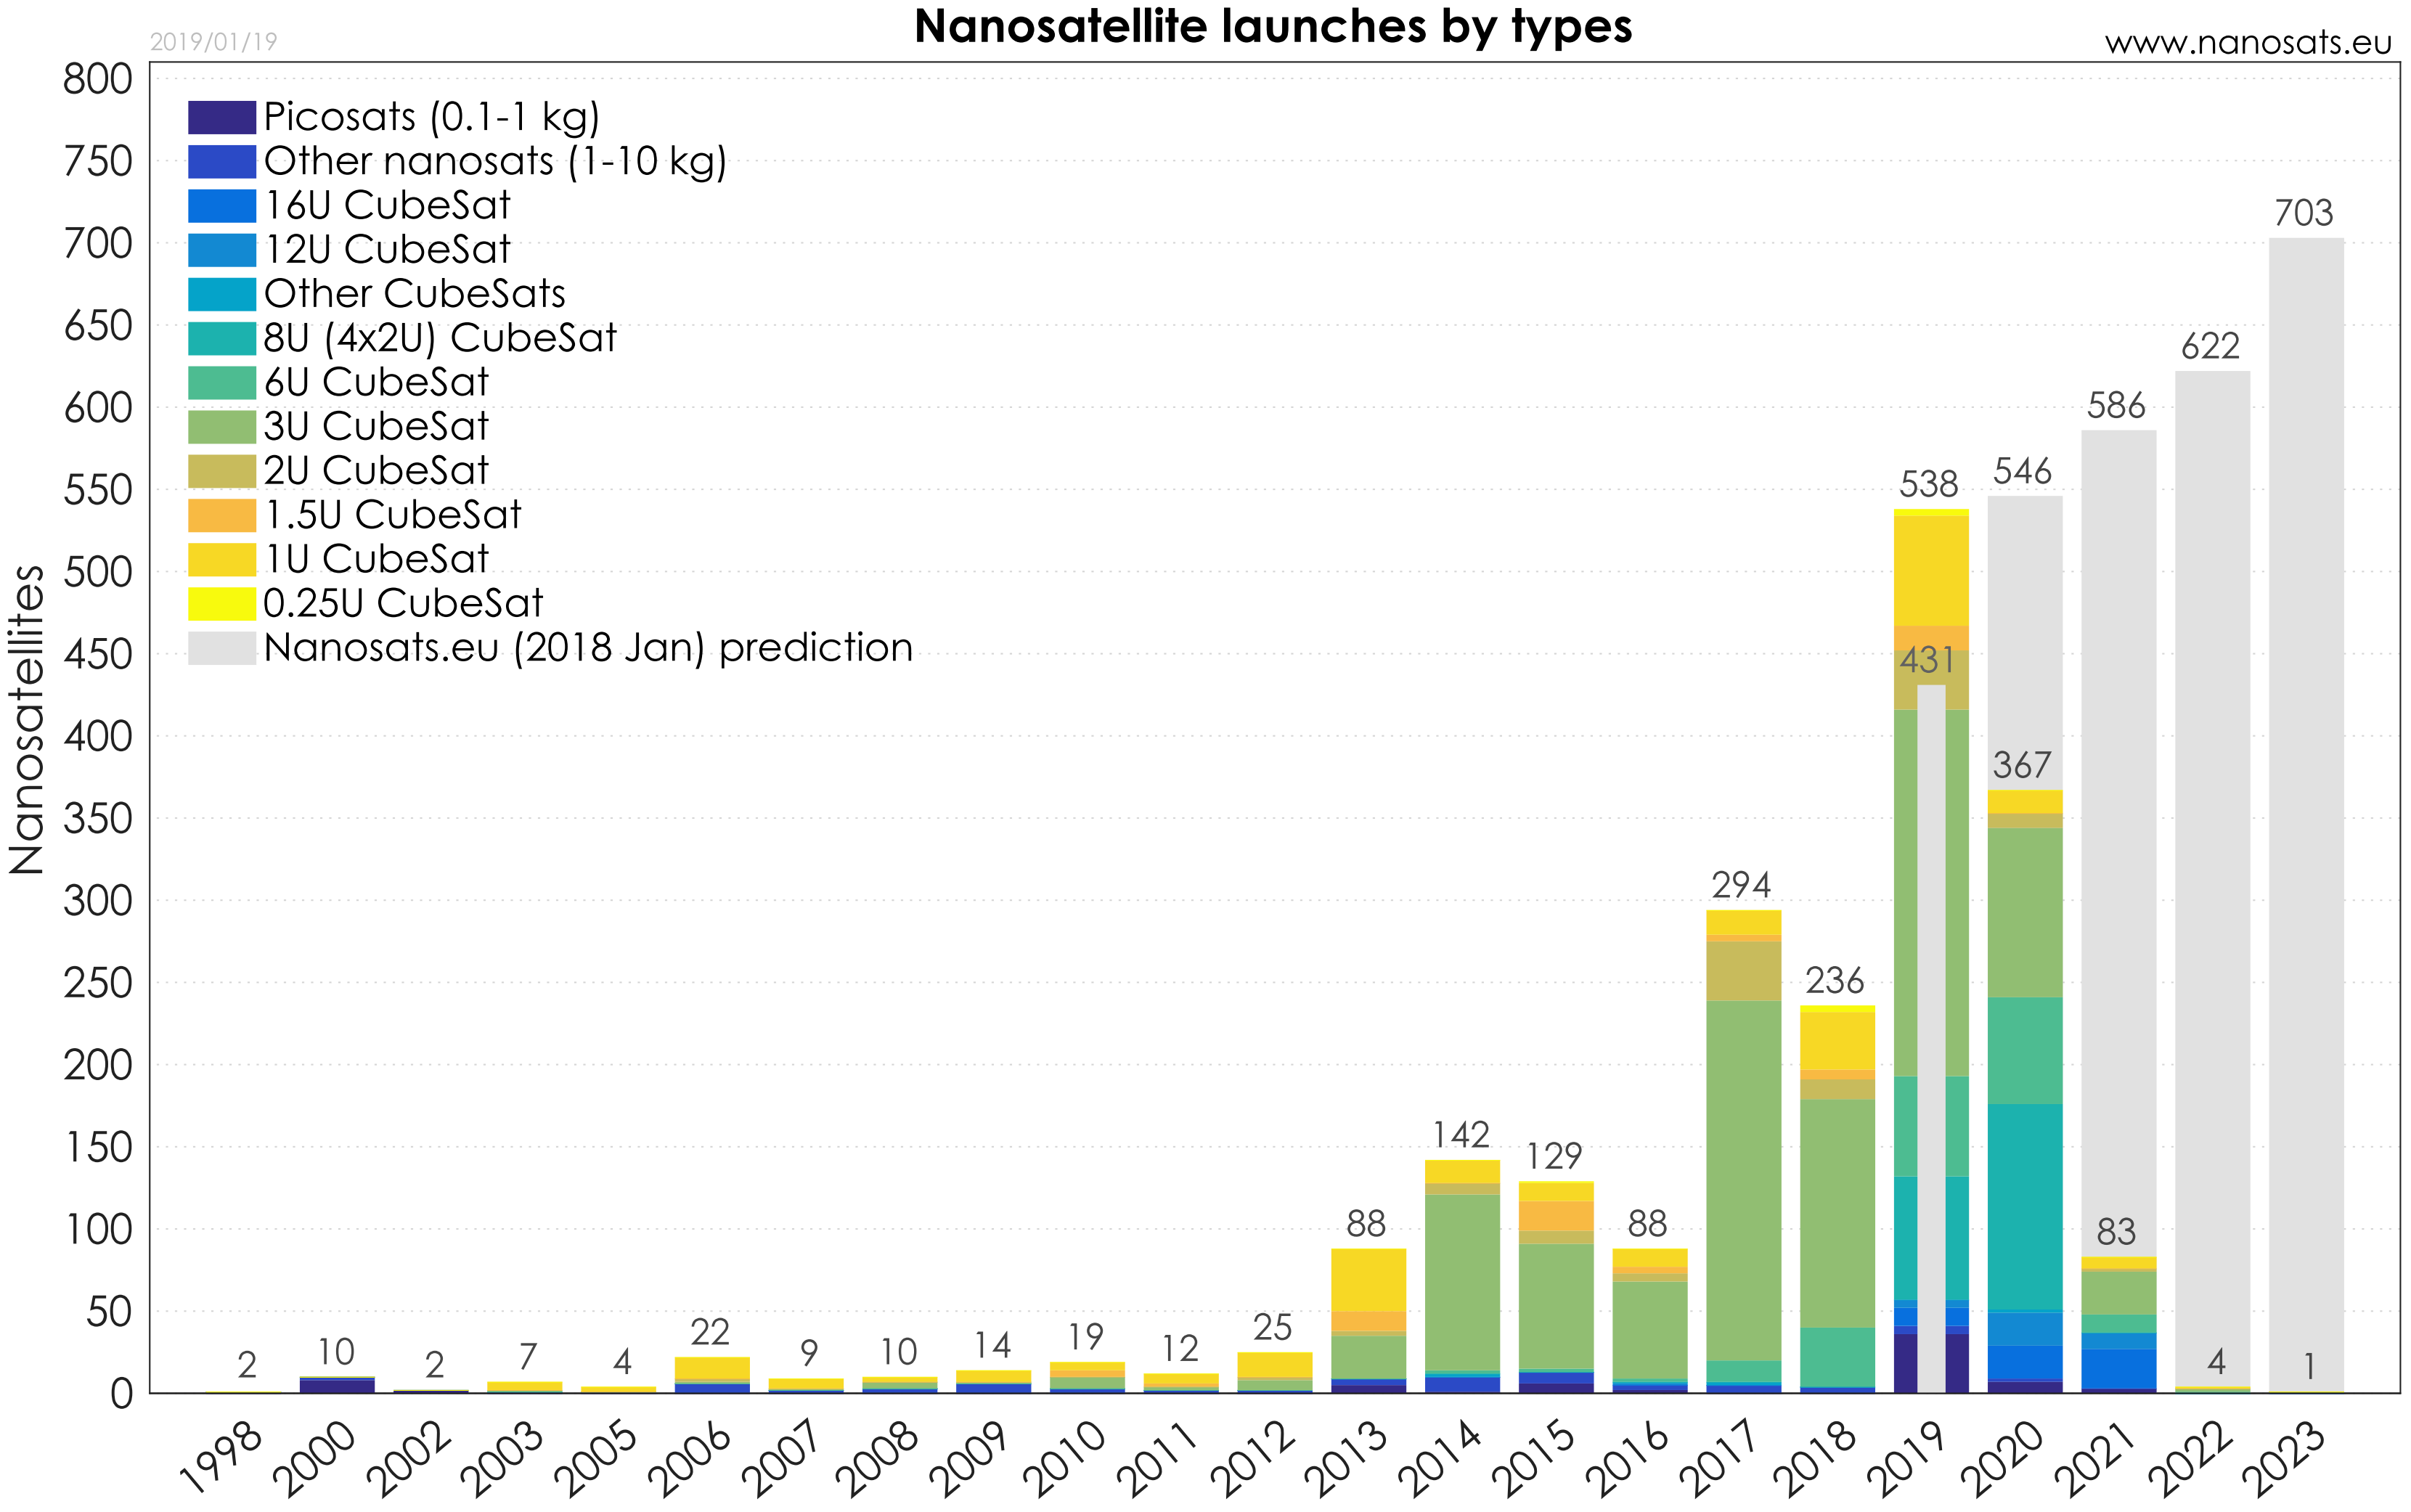
\includegraphics[width=0.80\textwidth]{Nanosats_years_types_2019-01-19_01}
				\caption{Überblick über Nanosatelliten Missionen von 1998 bis 2023 \cite{ErikKulu.2019}}
				\label{fig:NanosatsTypes}
			\end{figure}		
Die Fortschritte in der modernen Technologie unterstützen die Entwicklung der miniaturisierten Satelliten. Durch den Fokus der wissenschaftlichen Gemeinschaft auf Nano- und Picosatelliten sind die CubeSats zu einem wichtigen Teil der Kategorie geworden. Mit der Einführung des CubeSat-Konzepts 1998, welches zur Standardisierung von Masse und Größe von Satelliten führte, stieg die Zugänglichkeit des Weltraumes. Des Weiteren zeichnen sie sich durch ihre Modularität, leistungsstarken und kommerziell erhältlichen Satellitenkomponenten (commercial off-the-shelf) und ihren schnellen Entwicklungszyklen aus. Infolge der Standardisierung des CubeSats wurde das Startsystem Poly-Picosatellit Orbit Deployer (P-POD) entwickelt um eine kostengünstige Lösung für die Entwicklung und den sicheren Start bereitzustellen \cite[S. 1 - 4]{RahmatSamii.2017}. 2003 wurde die erste CubeSat Mission durchgeführt. Seitdem werden sie mit stark zunehmender Häufigkeit eingesetzt. Dies wird in \abb{fig:NanosatsTypes} veranschaulicht \cite[S. 1]{firstone}.  Hier werden in einem Säulendiagramm die durchgeführten, geplanten und vorhergesagten Nanosatelliten Missionen in dem Zeitraum von 1998 bis 2023 dargestellt. Aus dem Schaubild geht ab 2013 eine stetige Zunahme an CubeSat Missionen hervor. Auffallend ist der starke Zuwachs in dem Zeitraum 2018 bis 2019 mit einem Anstieg von  \num{236} Missionen auf \num{538} bei einer Vorhersage von \num{431} Missionen. Aus dem Diagramm lässt sich die Tendenz einer kontinuierlichen Zunahme von CubeSat Missionen seit ihrem Einsatz im Jahr 2003 erkennen. Dies liegt vorallem daran, dass eine große Zahl neuer Gruppen in die Weltraum-Erforschung eingestiegen ist, die Entwicklungszeit und Kosten einer Satelliten-Mission haben sich durch CubeSats enorm gesenkt \cite[S. 1 - 4]{RahmatSamii.2017}.
	
	%------------------------------------------------------------------------------------------------------------------------------------------------------------------------------
	\subsection[Gestaltungsrichtlinien]{Gestaltungsrichtlinien}
	\hfill\emph{(Frederik Schäfer)}\\
	Für die Gestaltung von CubeSats gelten eine Reihe von Richtlinien. Als kleinste Einheit (\SI{1}{\unit}) wird ein Würfel mit einer Kantenlänge von \SI{10}{\centi\metre} und einer zulässigen Masse von maximal \SI{1,33}{\kilogram} vorgegeben. Für größere Volumen und Massen können mehrere Einheiten von CubeSats verbunden werden. Satelliten mit \SI{1}{\unit}, \SI{1,5}{\unit}, \SI{2}{\unit}, oder \SI{3}{\unit} können von dem einheitlichen Startmechanismus (P-POD) in die Erdumlaufbahn ausgelassen werden. Die Kosten von CubeSat Missionen können gering gehalten werden, indem diese als sekundäre Nutzlast bei Raketenstarts mitfliegen. Für größere Satelliten (\SI{6}{\unit}, \SI{12}{\unit}, \SI{27}{\unit}) werden andere Startmechanismen benötigt \cite{Hevner.2011}. Die zugelassene Masse wird auf \SI[per-mode=symbol]{2}{\kilogram\per\unit} angehoben. Weitere Vorschriften gelten für die Folgenden Kriterien:
		\begin{itemize}
			\item \textit{Materialien:} 	\\ Alle bei der Konstruktion verwendeten Materialien müssen den Richtlinien der Air Force Space Command Manual entsprechen. Außerdem darf der Masseverlust des Satelliten durch verflüchtigende Materialien maximal \num{1}\% betragen.\cite{.c, CaliforniaPolytechnicStateUniversity.2014}
			\item \textit{Energiespeicher:} \\ Der chemische Energiespeicher darf eine Größe von \SI{100}{\watt\hour} nicht überschreiten.\cite{CaliforniaPolytechnicStateUniversity.2014} 
			\item \textit{Aktivierungszeitpunkt:} \\ Während der CubeSat im P-POD verstaut ist müssen alle Systeme ausgeschaltet bleiben. Beim Verlassen der Trägerrakete wird der Satellit aktiviert. Erst \num{30} Minuten später dürfen Bauteile (z.B. Solarpanele, Antennen, etc...) ausgefahren werden. Bevor die ersten Signale generiert oder gesendet werden müssen mindestens \num{45} Minuten vergangen sein.\cite{Hevner.2011} 
		\end{itemize}
		
		Falls ein Entwurf nicht den Vorschriften entspricht, kann bei dem Betreiber der Trägerrakete eine Sondergenehmigung angefragt werden. Nach einer Reihe von Tests entscheidet dieser ob er die Abweichungen akzeptiert, Änderungen vorgenommen werden müssen, oder ein anderer Anbieter gefunden werden muss. \cite{CaliforniaPolytechnicStateUniversity.2014} 

%-----------------------------------------------------------------------------------------------------------------------------------------------------------------------------
	\section{Cubesat Subsysteme}%-------------------------------------------------------------------------------------------------------------------------------------------
	%hier Hauptsächlich das Fazit von max kompakt darstellen und refernzieren
		\subsection{Antrieb}
\hfill\emph{(Florian Czorny)}\\
Eines der wichtigsten Subsysteme für Active Debris Removal (ADR) Missionen mit einem CubeSat ist der Antrieb. Er wird für Lageregelung und das Deorbiting des Zielobjekts benötigt.
Für CubeSats stehen nur wenige ausgereifte und erprobte Triebwerke zur Verfügung.  Die Miniaturisierung bestehender Technologien stellt eine große Herausforderung dar. Ein hoher TRL ist für die Auswahl besonders Entscheidend, da nur bereits erprobte Technologien für diese Mission genutzt werden sollten.
Im Wesentlichen lassen sich die Antriebsarten in chemische und elektrische Antriebe unterteilen.  Chemische Antriebe generieren im allgemeinen einen höheren Schub und werden für impulsive Manöver verwendet. Für den Betrieb muss ein großer Gewichtsanteil an Treibstoff einkalkuliert werden. Der spezifische Impuls ist jedoch deutlich niedriger als bei elektrischen Antrieben. Diese bieten auch ein besseres Schub-Leistungs-Verhältnis. Elektrische Antriebe sind jedoch auf eine ausreichende externe Energiequelle angewiesen. Diese wird zwangsläufig benötigt, um die getankte Masse zu beschleunigen.
Für genaue Untersuchung und den Vergleich der verschiedenen Triebwerkstypen wird auf die Literatur \cite{Lettau.} verwiesen. Miniaturisierte Versionen von erprobten Triebwerken werden stetig weiterentwickelt und getestet. Es wurden bereits mehrere Miniaturisierte Triebwerke in CubeSat-Missionen erfolgreich eingesetzt. 
%-----------------------------------------------------------------------------------------------------------------------------------------------------------------------------------
		\subsection[Stromversorgungssystem]{Stromversorgungssystem - Electrical Power System (EPS)}%----------------------------------------------------------------------------------------------------
\hfill\emph{(Frederik Schäfer)}\\
Das EPS ist für die Erzeugung-, Speicherung- und Verteilung von elektrischer Energie verantwortlich. 
Für die Stromerzeugung werden in der Raumfahrt hauptsächlich Solarpanele verwendet, welche auch für CubeSats die sinnvollste Lösung darstellen.
Für die meisten Anwendungen können Produkte verschiedener COTS-Anbieter erworben werden. CubeSats mit geringem Leistungsbedarf nutzen oft nur ihre eigene Oberfläche um mit Solarzellen Strom zu generieren. Wenn mehr Leistung benötigt wird werden faltbare Solarmodule eingesetzt. So kann die nutzbare Oberfläche zwei bis vier mal größer sein, als die benötigte Fläche auf dem Satelliten.\cite{Lettau.}

	Während der Satellit sich im Schatten der Erde befindet wird Energie aus einem internen Speicher genutzt. Dieser besteht in der Regel aus Lithium basierten Akkus, welche eine hohe Energiedichte von bis zu \SI[per-mode=symbol]{240}{\watt\hour\per\kilogram} aufweisen. Sie können sowohl als einzelne Zellen, als auch in vorgefertigten Paketen von COTS-Anbietern erworben werden.\cite{Lettau., Abaker.2017}
	

%\begin{figure}[!h]                              \SI{}{\kilogram}
	%\centering
		%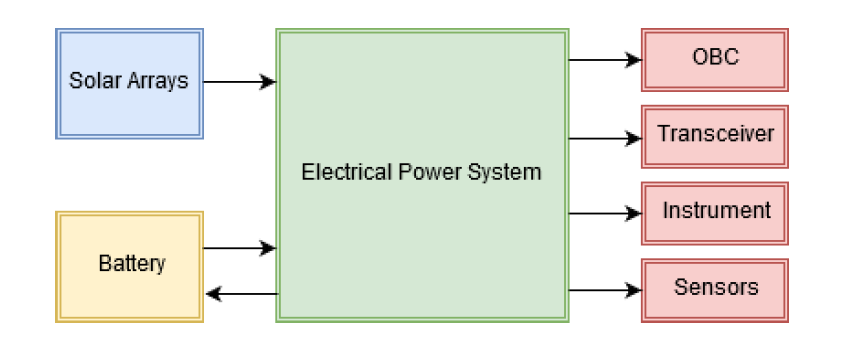
\includegraphics[width=0.50\textwidth]{./graphics/Struktur_EPS.PNG}
	%\caption{EPS Aufbau \cite{Pelgrift.2017}}
%\end{figure}

	Für die Verteilung des Stroms an die Subsysteme gibt es zwei unterschiedliche Ansätze. Zum Einen sind es dezentralisierte Verteilungssysteme [Abb. \ref{d_eps}], die ein modulares und flexibles Design erlauben. Dieses kann für verschiedene Satelliten angepasst werden. Es arbeitet mit nur einer Ausgangsspannung, die dann für jedes angeschlossene Subsystem einzeln umgewandelt wird.%ggf mikrospannungswandler erklären nach Burt.2011
\begin{figure}[t]
	\centering
		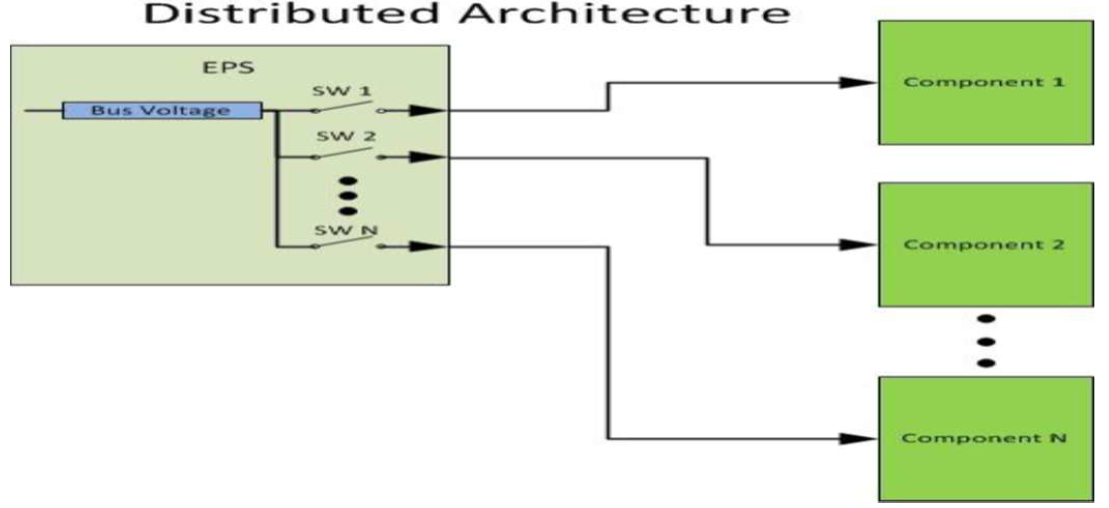
\includegraphics[width=0.50\textwidth]{./graphics/Distributed_EPS.PNG}
	\caption{Dezentralisiertes EPS \cite{Burt.2011}}
	\label{d_eps}
\end{figure}

 Die zweite Variante sind zentralisierte Verteilungssysteme [Abb. \ref{c_eps}]. Diese werden häufiger verwendet, da sie den Vorteil eines geringen Volumens bieten und weniger Spannungsregler benötigen. Das wird erreicht, indem alle Subsysteme mit gleicher Spannung am selben Regler angeschlossen werden. Nachteilig ist, dass dieser Regler auf die maximale Gesamtlast aller Subsysteme ausgelegt werden muss. Das führt dazu, dass zentralisierte Systeme zwar im Aufbau einfacher ausfallen, jedoch aufgrund der Maximallastauslegung weniger effizient sind.\cite{Abaker.2017}
\begin{figure}[H]
	\centering
		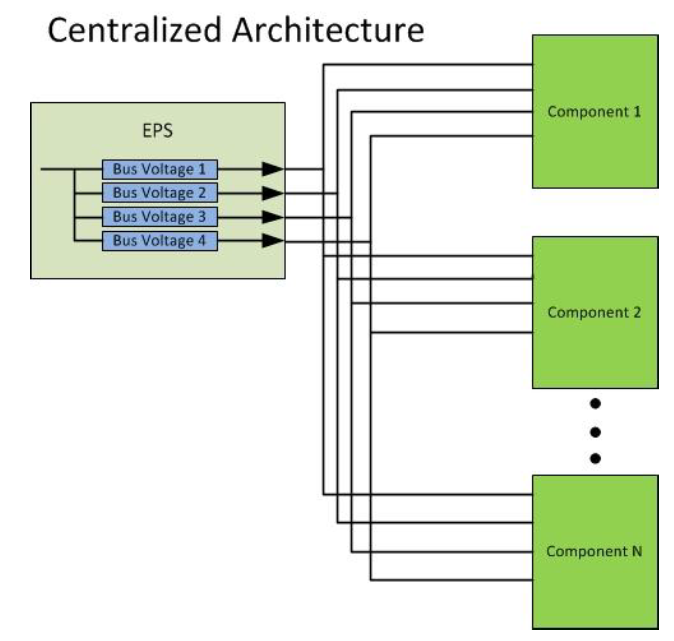
\includegraphics[width=0.50\textwidth]{./graphics/Centralized_EPS.PNG}
	\caption{Zentralisiertes EPS \cite{Burt.2011}}
	\label{c_eps}
\end{figure}



		%-----------------------------------------------------------------------------------------------------------------------------------------------------------------------------
		\subsection{Guidance, Navigation and Control}
		\hfill\emph{(Oussama Mouhaya)}\\
Guidance, Navigation and Control (GNC) Subsysteme sind neben den in Kapitel [2.2] genannten Systemen unabdingbar für ADR Missionen, da diese die Positionsbestimmung als auch die Lagebestimmung und Regelung beinhaltet. Dieses System kann in zwei Hauptbereiche unterteilt werden: der Lage- und Positionsbestimmung, sowie der Lageregelung.
Bei der Lage und Positionsbestimmung kann auf verschiedene Sensoren zurückgegriffen werden. Die absolute Positionsbestimmung erfolgt über eine Bodenstation, welche auch zur Kommunikation mit dem Satelliten verwendet wird. Bei dieser Art der Positionsbestimmung ist es notwendig zu wissen, welchen geplante Erdumlaufbahn der Satellit hat. Diese Methode bezieht sich auf der Zeitdifferenz zwischen Sende- und Empfangszeitpunkt. Deswegen ist die Positionsbestimmung via Bodenradar nicht sehr genau \cite{.d}. Seit der erfolgreichen Miniaturisierung  von GPS Empfängern werden auch diese zur Positionsbestimmung verwendet. Dies funktioniert solange die GPS Satelliten die Einsatzhöhe von CubeSats überschreiten. Die Lagebestimmung über Startracker erfolgt in dem ein Bild des Himmels mit einem Katalog abgeglichen wird. Dadurch kann die Lage bei bekannter Position bestimmt werden. Weitere Möglichkeiten sind Sonnen-, Erd- Magnetfeldsensoren, sowie Kreiselinsturmente. Bei Kreiseln wird die Verdrehung im Vergleich zu einem aufgeprägten Inertialsystem gemessen, wodurch die Lage genau bestimmt werden kann. 
Die Regelung  der Lage kann über unterschiedliche Methoden erfolgen. Die einfachste ist eine Drehbewegung um eine der Hauptachsen. Dies führt zu einer Stabilisierung des Satelliten, ist jedoch für eine CubeSat, dessen Aufgabe das Docking und deorbiting beinhaltet, nicht sinnvoll. Dementsprechend kann eine 3 achs-Stabilisierung durchgeführt werden, welche durch Triebwerke und Reaktionsräder durchgeführt werden kann. Diese Art der Lageregelung benötigt ein Reaction Control System (RCS) um unkontrollierte bewegungen zu vermeiden. Die Regelung mittels RCS-Triebwerken geschieht indem Schubimpulse in die jeweilige Richtung gegeben werden. An allen drei Hauptachsen sind Schwungräder montiert. Durch den Antrieb der Räder wird ein Moment erzeugt welches den Satelliten in die gewünschte Lage bringt. Da ein 3-achs System nicht nur Stabilisiert, sondern auch die gewünschte Lage herbeiführen kann, ist dieses System für den viele Fälle optimal.\cite{Lettau.}

%------------------------------------------------------------------------------------------------------------------------------------------------------------------------------
		\subsection{Command und Data Handling}%-------------------------------------------------------------------------------------------------------------------------------------
		\hfill\emph{(Marc Strempel)}\\
		Das Command- und Data-handling Subsystem (CDHS) ist die Prozessoreinheit, die sich um alles kümmert was mit Software gesteuert wird. Hier werden Daten zu allen Subsystemen und Nutzlasten gesammelt. Das CDHS stellt die Daten bereit, die übertragen werden sollen und führt Befehle aus, die an das Kommunikations Subsystem gesendet werden. 
Es sorgt für die korrekte Einstellung der Solarzellen und Ladung der Batterien. Alle Berechnungen zur Position in der Erdumlaufbahn und der aktuellen Zeit finden hier statt. Neben dem aktiven Ausführen von Befehlen beobachtet und löst der Prozessor eine Reihe an Problemen, die während der Mission auftreten können. Die Bestandteile des CDHS sind der Raumflugrechner, die Flugsoftware und ein Speichermedium.\cite{Lettau.}

%--------------------------------------------------------------------------------------------------------------------------------------------------------------------------------
		\subsection{Kommunikation}%-----------------------------------------------------------------------------------------------------------------------------------------------
		\hfill\emph{(Marc Strempel)}\\
Das Kommunikations Subsystem sorgt bestenfalls für eine dauerhafte Verbindung zur Bodenstation. Aufgezeichnete Daten und eingehende Befehle werden hier von, und an den Cubesat übertragen. Das Subsystem besteht aus den Telemetrie- und Befehlsystemen.
Das Telemetriesystem besteht aus einem oder mehreren Transmittern, welche die vom Prozessor kommenden Daten als Signal an die Bodenstation über die Antennen an Bord des Cubesats aussenden. Die Signale werden als Mikrowelle übertragen und empfangen. Je nach verwendetem System handelt es sich dabei um S-Band-, oder X-Band Wellen. Wellen im X-Band Spektrum können zwar, aufgrund der höheren Frequenz, höhere Bandbreiten erreichen, aber die Technologie ist noch nicht so etabliert wie S-Band Transmitter.\cite{Lettau.}
		
		%---------------------------------------------------------------------------------------------------------------------------------------------------------------------------
		\subsection{Thermisches Management}%------------------------------------------------------------------------------------------------------------------------------------------------------
		\hfill\emph{(Valentina Dietrich)}\\
Die Wärmeübertragung im Vakuum erfolgt ausschließlich durch Wärmeleitungen und Strahlungen. Das Wärmemanagement regelt den Bereich der zulässigen Temperaturen für die Sicherstellung einer optimalen Funktionalität und das Überleben des Satelliten. Hier unterscheidet man zwischen passiven und aktiven Methoden des thermischen Management  Durch die Massen-, Volumen- und Leistungsbeschränkungen bei miniaturisierten Satelliten, wie dem CubeSat, liegt der Fokus auf den passiven Wärmereglungstechnologien, da die Fortschritte bei der Entwicklung von miniaturisierten aktiven Wärmeregelungsmethoden begrenzt sind. Passive Technologien sind mit geringen Kosten, Volumen, Gewicht und Risiko verbunden und erfordern keine interne Eingangsleistung für die Wärmeregulierung. Thermische Beschichtungen, Wärmerohre, Sonnenschirme, Wärmebänder und Multi-Layer Insulation (MLI) sind passive Methoden für die Regulierung des thermischen Gleichgewichtes. Die aktiven Methoden, wie elektrische Widerstandsheizungen, Kühler oder kryogene Materialien, sind mit höherer Präzision und interner Eigenleistung verbunden. Die Verwendung von aktiven Systemen ist bei temperaturempfindlichen Geräten und nicht ausreichender passiver Systeme für eine Aufrechterhaltung der Betriebstemperatur vielversprechender. \cite[S. 109 - 120]{NASA.Sota.2018} 

%------------------------------------------------------------------------------------------------------------------------------------------------------------------------------
		\subsection{Struktur}%-------------------------------------------------------------------------------------------------------------------------------------------
		\hfill\emph{(Valentina Dietrich)}\\
Die Strukturen werden in Primär- und Sekundärstrukturen unterteilt. Die Primärstruktur ist thermischen und dynamischen Einflüssen ausgesetzt, denen sie standhalten muss. Weiterhin dient sie der Lastübertragung während des Starts und des Einsatzes. Elektromagnetische Strahlung, Druck und innere Wärmeleitung sind weitere Faktoren, die einen großen Einfluss auf das Gehäuse haben und deshalb mit einbezogen werden müssen. Die Begrenzungen bei der Oberfläche und bei dem Volumen sorgen für Einschränkungen. Infolgedessen sollte die Struktur effizient ausgelegt werden. Komponenten, die nur sich selbst tragen müssen, wie Sonnenkollektoren, zählen zu den Sekundärstrukturen auf die nicht näher eingegangen wird, da sie bei einem Ausfall die Integrität des Raumfahrzeugs nicht beeinträchtigt. Die Primärstrukturen werden als COTS-Strukturen und kundenspezifisch bearbeitet oder gedruckte Komponenten auf dem Markt angeboten. Generell besteht das Gehäuse aus metallischen und nichtmetallischen Materialien und wird von der Betriebsumgebung des Satelliten bestimmt. \cite[S. 96 - 108]{NASA.Sota.2018} 

%------------------------------------------------------------------------------------------------------------------------------		
	\section{ADR Mission}
		\hfill\emph{(Oussama Mouhaya)}\\
Eine ADR Mission setzt sich aus verschiedenen Abschnitten zusammen. In diesem Kapitel werden einige verwendbare Methoden aufgelistet und eingegangen. Anschließend wird der kritische Punkt des Rendezvous Betracht und einzelnen Phasen näher betrachtet. Anschließend wird auf das Docking näher erleuchtet und auf das adhäsive Docking mittels Geckomatrialen  eingegangen. 
%------------------------------------------------------------------------------------------------------------------------------
\subsection{ADR Methoden}
\label{ADRm}
%------------------------------------------------------------------------------------------------------------------------------
	
	Für eine ADR Mission gibt es verschieden Methoden um diese durchzuführen. Die Grafik \ref{fig:ADR_Methoden} zeigt unterschiedliche Cluster von ADR Methoden, welche unterschiedliche Vor-und Nachteile, sowie TRL haben. Im Folgenden wird auf jedes Cluster eingegangen, beschrieben und den aktuellen Status erläutert.
	
				\begin{figure}[h]
				\centering
					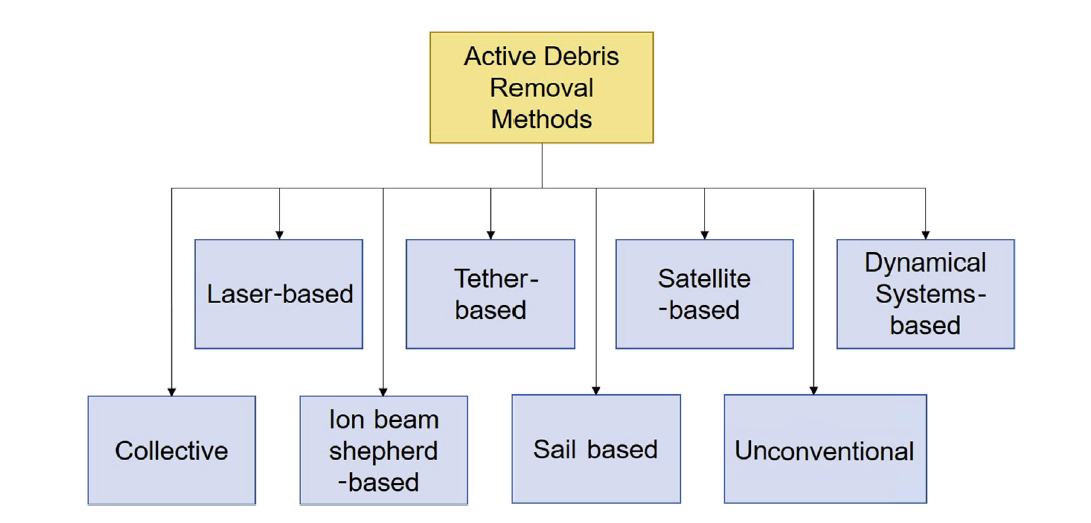
\includegraphics[width=0.80\textwidth]{./graphics/ADR/ADR_methods.PNG}
				\caption{Überblick über die ADR Methoden \cite{Mark.2019}}
				\label{fig:ADR_Methoden} 
			\end{figure}
			
	
Es gibt einige Herausforderungen, welch unabhängig von der Removal Methode sind und für jede Mission individuell gelöst werden muss. Dazu gehört die Klassifizierung der zu entfernenden Objekte, sowie dessen genaue Positionsanalyse. Sollen während einer Mission mehrere Objekte entfernt werden, so muss zu beginn definiert werden in welcher Reihenfolge dies geschehen soll. 

%---------------------------------------------------------------------------------------------------------------------
	\subsubsection{Collective Method}
%----------------------------------------------------------------------------------------------------------------------	
	
				\begin{figure}[h]
			\centering
					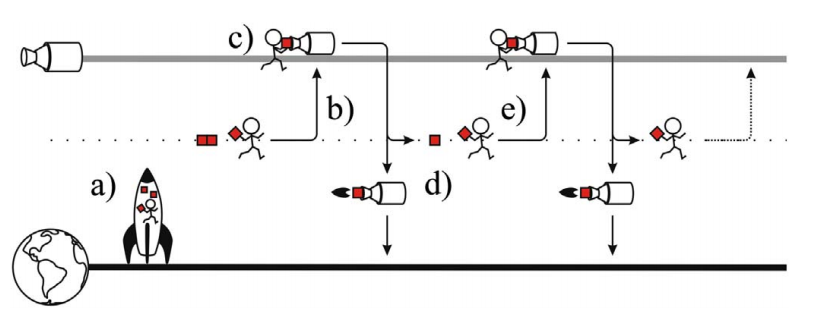
\includegraphics[width=0.80\textwidth]{./graphics/ADR/collective_method.PNG}
				\caption{Missionsaufbau für Collective Method \cite{Peters.2016}}
				\label{fig:Sammelmethoden}
			\end{figure}
	
	
Die Abbildung \ref{fig:Sammelmethoden} zeigt den grundlegenden Aufbau eine ADR Mission welche auf ein Sammelverfahren beruht. Dabei wird ein Satellit mit Deorbiting Kits ausgestattet, welcher die verschieden Ziele anfliegt und diese anbringt. Ein großer Vorteil ist, dass nur ein Trägersatellit mit anspruchsvoller Technik für die Navigation, Positionsbestimmung, Dockingmechnismen und Energieversorgung ausgestattet werden muss. Da der Trägersatellit mehrere Ziele anfliegt, muss dieser über ein sehr großes Tankvolumen verfügen, da möglicherweise mehrere Orbithöhenanpassungen  durchgeführt werden müssen. Neben der Orbithöhe muss vermutlich auch eine Änderung der Inklination und Exzentrizität durchgeführt werden. Dies kann auch bei kleinen Unterschieden der Variablen zu einem sehr hohen Treibstoffverbrauch führen. Außerdem wird bei jedem Zielobjekt ein Rendezvous Manöver sowie Docking durchgeführt, welche das Potential haben durch eine Kollision weiter Trümmer zu erzeugen \cite{Peters.2016, Mark.2019}.

%------------------------------------------------------------------------------------------------------------------------
			\subsubsection{Laser-based Method}
%-----------------------------------------------------------------------------------------------------------------------
	
	Wie der Name es bereit sagt beruht diese Methode auf Laser , welcher sich auf der Erde befindet. Es wird ein hochenergetischer Laser benötigt, welcher in einer geringen Zeit das Objekt befeuert. dadurch entsteht ein Plasmastrahl, welcher den Satelliten bremst und dadurch eine Verringerung der Orbithöhe resultiert. Dieses System kann dazu verwendet werden um sowohl große als auch kleine Objekte zu entfernen, sowie dessen kosteneffizient. Das größte Problem bei dieser Methode, ist die Zielfindung und Verfolgung. Damit das deorbiting funktioniert muss der Laser für ein bestimmtes Zeitinkrement auf das Ziel gerichtet sein, was eine genau Berechnung der Zielposition in Abhängigkeit der Dauer von Start des Laserstrahls und erreichen des Ziels.\cite{Phipps.2012,Mark.2019}

%-------------------------------------------------------------------------------------------------------------------------
\subsubsection{Ion beam shepherd-based Method}
%-------------------------------------------------------------------------------------------------------------------------
	\begin{figure}[h]
			\centering
					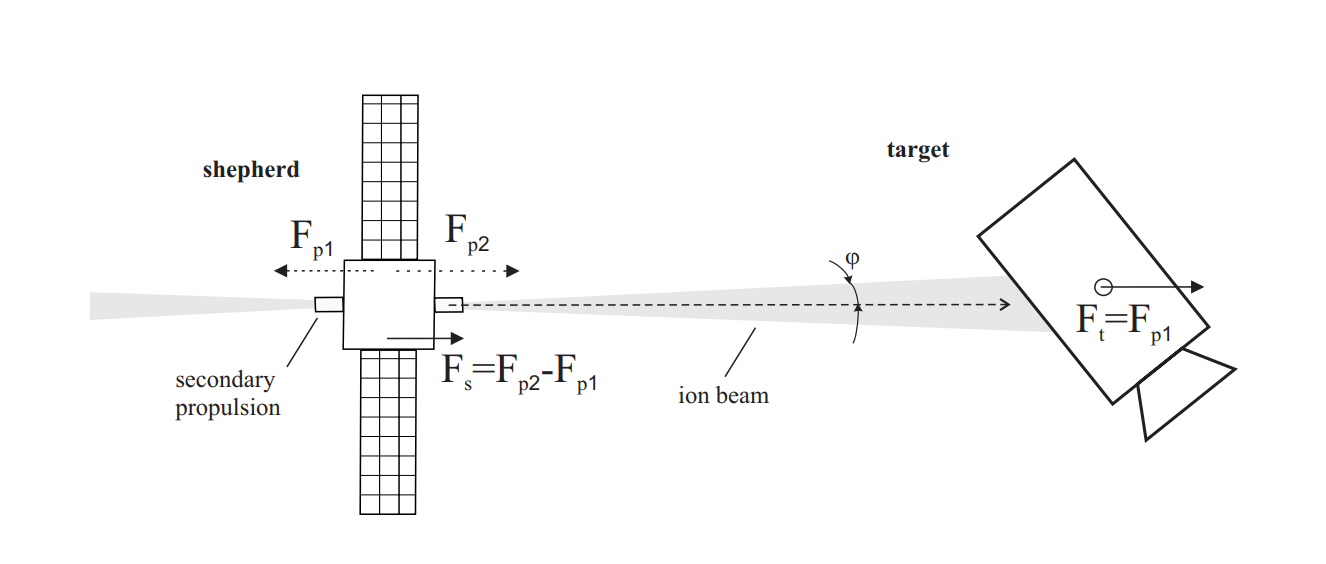
\includegraphics[width=0.80\textwidth]{./graphics/ADR/Shepherd.PNG}
				\caption{Funktionsweise des ADR mittels Laser \cite{Bombardelli.2011}}
				\label{fig:Laser}
			\end{figure}

	
Die Abbildung \ref{fig:Laser} zeigt den schematischen Aufbau einer ADR Mission nach Ion Based Shepherd Methode. Der Chaser Fliegt vor dem Zielobjekt und bremst diesen durch ein Ionenstrahl aus dem zum Objekt gerichteten Triebwerk. Besonders zu beachten ist die Streuung des Ionenstrahl und die genaue Positionierung des Chasers vor dem Zielobjekt \cite{Mark.2019}.

%---------------------------------------------------------------------------------------------------------------------------
\subsubsection{Tether Based Methode}
%----------------------------------------------------------------------------------------------------------------------------
	
	Diese Methode des deorbiting beruht auf dem fangen/ festhalten von Objekten. Betrachtet werden dabei primär Fangnetze und Harpunen. Problematisch ist bei beiden Systemen die Simulation der dynamischen Bewegungen im Orbit. Es wurden bereits Experimente diesbezüglich durchgeführt. Die Kontrolle des Fangmeschnismusses und des Zielobjekts sind aktuelle Themen der Forschung. Bei Harpunen ist ein weiterer Risikofaktor der Einschlag. Es besteht die Möglichkeit der Beschädigung des Satelliten und dadurch resultierend eine Zerstörung \cite{Mark.2019}.
%--------------------------------------------------------------------------------------------------------------------------------------
\subsubsection{Sail based Method}
%--------------------------------------------------------------------------------------------------------------------------------------

	\begin{figure}[h]
			\centering
					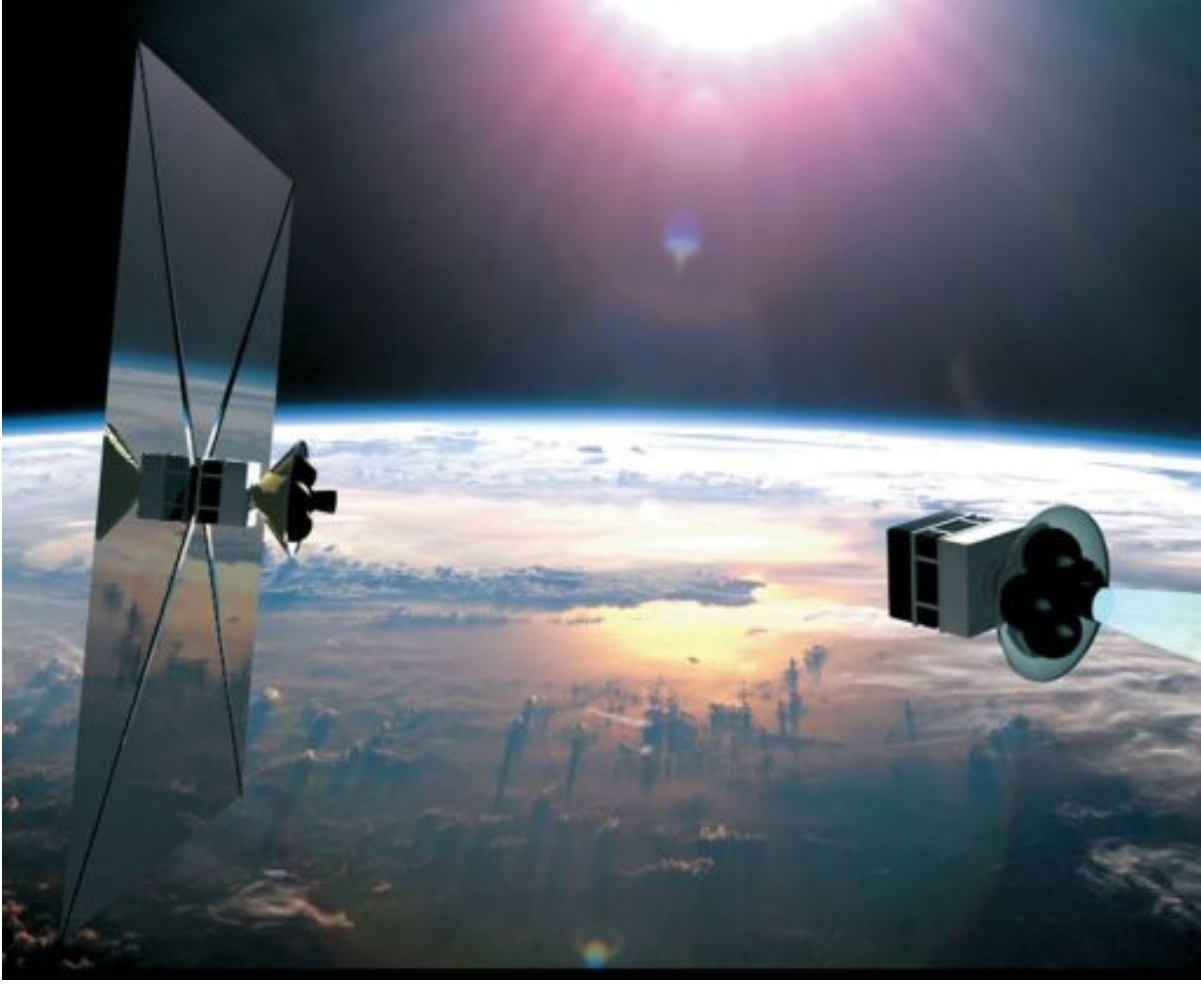
\includegraphics[width=0.60\textwidth]{./graphics/ADR/Sonnensegel.PNG}
				\caption{Satellit mit Sonnensegel \cite{Romagnoli.2012}}
				\label{fig:Segel}
			\end{figure}

	
Wie in der Abbildung \ref{fig:Segel} zu erkenne, wird ein Sonnensegel verwendet um den Nötigen Schub zu erzeugen. Unschwer zu erkennen, ist das ein Sonnensegel im Verhältnis zu dem Satelliten sehr groß ist. Diese Fläche ist Notwendig, um einen Solarenstrahlungsdruck zu generieren welcher eine Veränderung der Geschwindigkeit herbeiführt. Eine Hauptaufgabe beim Entwickeln dieses Systems ist die Größe und die Auslegung des Segels, und damit zusammenhängend der komplexe Faltmechanismus. Des weiteren ist diese Art des Deorbiting langsam und Unkontrolliert. Da die Geschwindigkeitsänderung über den Strahlungsdruck der Sonne generiert wird, muss kein weiteres Gewicht inform von einem Antrieb oder Zusatztreibstoff für das deorbiting mitgenommen werden \cite{Romagnoli.2012,Mark.2019}.

%----------------------------------------------------------------------------------------------------------------------------------------
\subsubsection{Satellite based Method}
%----------------------------------------------------------------------------------------------------------------------------------------
	
	Die bereits genannten Methoden beruhen teilweise auf Satelliten. Ziel bei dieser Methode ist nicht die Entwicklung eines neuen ADR- Systems, sondern die Optimierung und Miniaturisierung der bereits angesprochen Methoden. Dies ist ein großer Vorteil, da auf basis eines Satelliten verschiedene Methoden getestet und durchgeführt werden könne. Die Spanne der Einsatzmöglichkeiten geht hierbei von der Collective Methode mit dem Warehouse-system bis hin zu einmal Satelliten. Jedoch ist ein Satellit im Vergleich zu anderen Systemen komplex und die Leistung muss gesteigert werden. Obwohl diese Art von Satelliten nicht mit einer eigenen Rakete gestartet werden ist es sehr kostspielig einen Satelliten in den Orbit zu befördern. Diese Art des Deorbiting erfordert ein hohen Autonomiegrad, da sowohl das Rendezvous als auch das Docking Autonom erfolgen muss \cite{Mark.2019}.

	\begin{figure}[h]
			\centering
					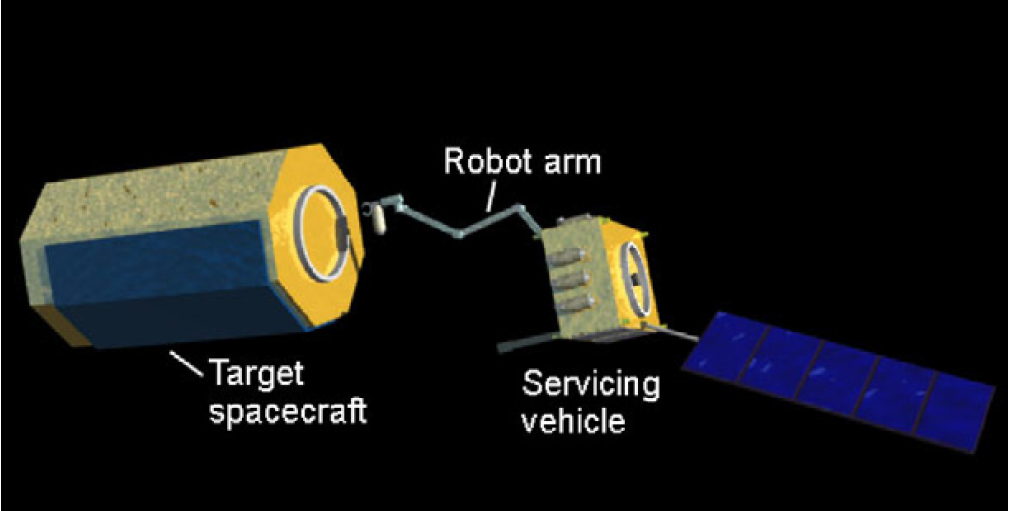
\includegraphics[width=0.60\textwidth]{./graphics/ADR/Sattelit_Methode.PNG}
				\caption{Satellit mit Roboterarm \cite{Nishida.2011}}
				\label{fig:Satellit}
			\end{figure}
			
	
%-------------------------------------------------------------------------------------------------------------------------------------------
\subsubsection{Unconventional	Method}
%-------------------------------------------------------------------------------------------------------------------------------------------
	
	Diese Methoden sind von Grundlegenden Konzept keine der Kategorien zuzuordnen sind. Beispielhaft zu nennen ist die Erzeugung eines Magnetfeldes welches von dem Objekt generiert wird und durch die Interaktion mit dem Erdmagnetfeld eine Reduzierung der Orbithöhe zufolge hat. Diese Methoden sind unkonventionell und liefern neue Ideen für ADR-Missionen. In der Theorie sind diese sehr effektiv, aber nicht Umsetzbar \cite{Mark.2019}.
					
%------------------------------------------------------------------------------------------------------------------------------		
	\subsection{Rendezvous} 
		\hfill\emph{(Oussama Mouhaya)}\\
%------------------------------------------------------------------------------------------------------------------------------
	\begin{figure}[h]
			\centering
					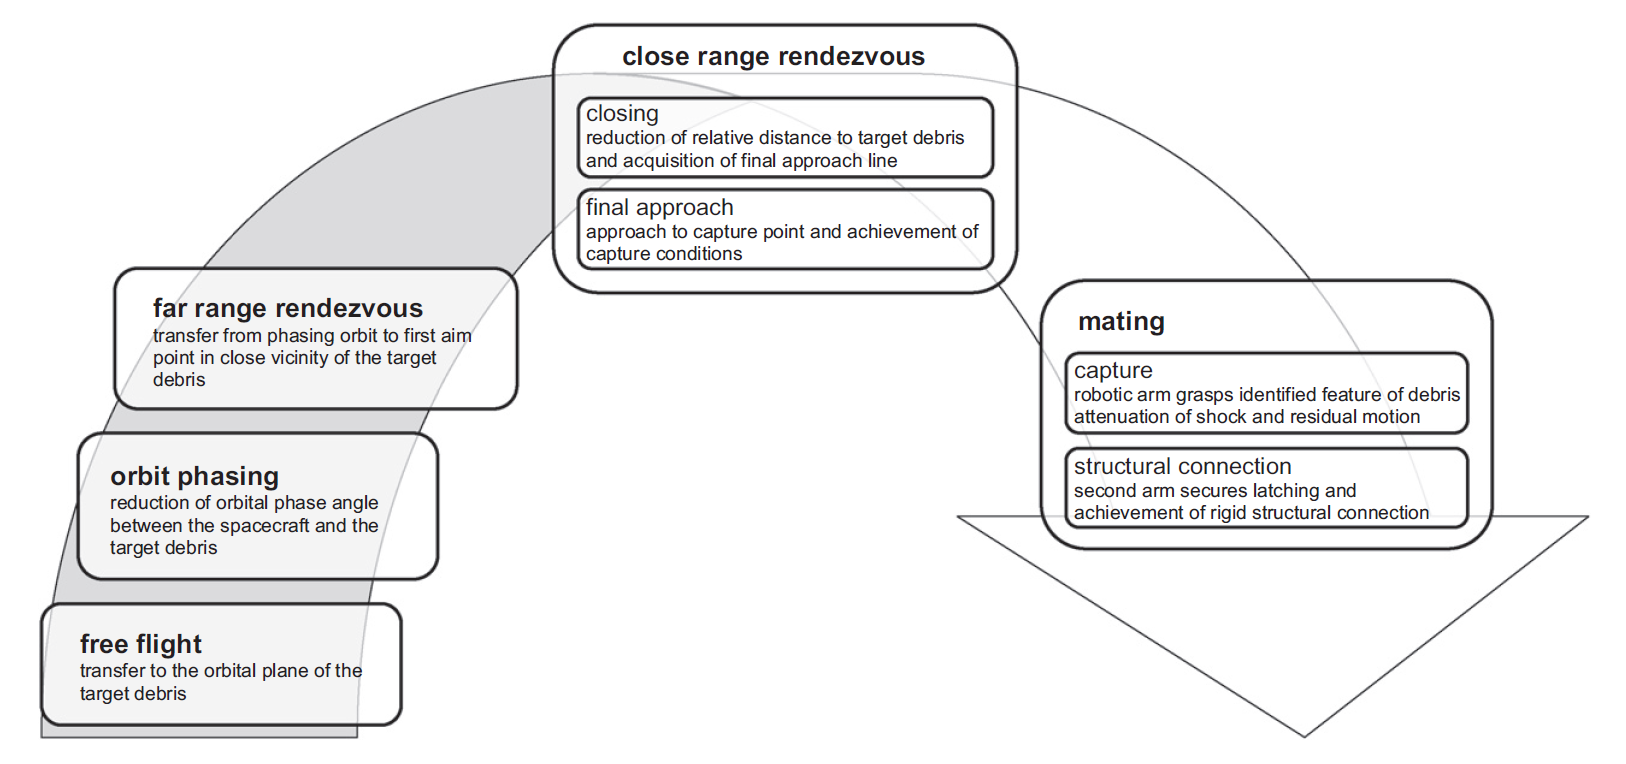
\includegraphics[width=0.80\textwidth]{./graphics/ADR/Rendezvous.PNG}
				\caption{Rendezvous Phasen\cite{Castronuovo.2011}}
				\label{fig:Rendezvous}
			\end{figure}
Rendezvous ist ein kritischer Missionsabschnitt bei einer ADR Mission. Wie in der Abbildung \ref{fig:Rendezvous} zu erkennen, ist dieser Missonsabschnitt wiederum in verschiedene Phasen unterteilt. In der ersten Phase, dem Free Flight, wird wenn notwendig ein Orbittransfer durchgeführt. Dabei nähert sich der Chaser dem Zielorbit und synchronisiert sich mit dessen Inklination. Die Orbithöhe des Chasers ist unterhalb der Zielhöhe, um eine Annäherung zu gewährleisten, da Satelliten mit einer niedrigeren Orbithöhe eine höhere Geschwindigkeit haben. Bei der Orbit Phase wird die Höhendifferenz reduziert, bis der Chaser ca. 5 km hinter und 1 km unterhalb des Ziels ist. Ab diesem Punkt beginnt die Far Range Rendezvous Phase. In dieser Phase wird die relative Navigation verwendet, welche auf Sensoren und Aktuatoren zurückgreift die in Kapitel 2.2 beschrieben worden sind. Besonders LIDAR und Kamera-Systeme werden in dieser Phase benötigt, da die absolute Navigationssysteme nicht die nötige Genauigkeit liefert und eine Kollision dem Ziel der Mission widerspricht und zu einer Verschlimmerung der Problematik führt. Diese Phase endet bei ca. 100 m Entfernung zwischen Ziel und Chaser. Nun beginnt das Close Range Rendezvous, welches die Closing Phase und den Final Approach beinhaltet. Vor der Closing Phase wird das Objekt genau betrachtet, es werden alle relevanten Informationen Über das Ziel gesammelt und verglichen, dies beinhaltet auch die genaue Taumelbewegug und deren Beschreibung. Dabei wird darauf geachtet ob eine Rotationsachse vorhanden ist und wie die Beschaffenheit der Oberfläche ist. Sollte eine Taumelbewegung vorhanden sein, wird der Chaser mit dieser Synchronisiert. Nach der Synchronisierung findet das Closing und der Final Approach statt, in dem die Distanz weiter reduziert wird und schlussendlich das Docking durchgeführt wird \cite{Castronuovo.2011}. 
 
%------------------------------------------------------------------------------------------------------------------------------
		\subsection{Docking Strategien}
			\hfill\emph{(Oussama Mouhaya)}
%------------------------------------------------------------------------------------------------------------------------------		

\subsubsection{Roboterarm}

	Die Docking Strategien sind meist die Grundlage für die bereits beschrieben ADR Konzepte.	Da ein Dockingmanöver nur bei  Missionen durchgeführt wird, bei denen das Satellitenbsierte ADR Konzept verwendet wird notwendig ist, wird hier nur auf spezielle Systeme eingegangen. Eines der ersten Strategien ist der Roboterarm, dabei wird wie erwähnt ein Roboterarm an einen Satelliten montiert. Dises System ist nicht nur auf einen beschränkt, sondern kann mit beliebig vielen weiten Modulen Versehen werden. Limitieren sind hierbei nur das Volumen und die benötigte Energie. Zu beachten ist, dass mit steigender Anzahl an Modulen auch die Anforderungen an das RCS-System sowie des Messsensorik. Das Docking erfolgt wie in \ref{fig:Satellit} gezeigt. Der Roboterarm wird nach dem Final Approach an dem Zielobjekt befestigt, wodurch eine Verbindung zwischen Zielobjekt und Chaser hergestellt wird. Diese Form des Docking ist etwas weniger Risikoreich als es beim Adhäsivem Docking ist, da kein direkter Kontakt zwischen beiden Satelliten besteht. Jedoch macht dies auch eine Aufwendige Steuerung für den Roboterarm notwendig \cite{Castronuovo.2011}.

\subsubsection{Fangnetz}

	Ein Docking mit Fangnetzen ist technisch aufwendig, da die Bewegung nicht mit absoluter Sicherheit berechnet werden kann und es besteht die Gefahr des Verknotens. Des weiten ist die Regelung eines so dynamischen Systems sehr komplex und die Manövrierfähigkeit ist eingeschränkt. Da das System keine feste Verbindung hat, sind unkontrollierte Bewegungen möglich welche die Struktur den Netzes, des Zielobjekts und des Satteliren beschädigen können. Auch wenn bereits Konzepte mit Netzen bei Parabelflügen getestet wurden, sind weiterführende  Forschungen notwendig, um das Potential dieser Methode zu erhöhen


\subsubsection{Adhäsiv Docken}

	Das adhäsive Docking beruht auf dem System einer Klebverbindung. Dafür unerlässlich ist der Kontakt zwischen zwei Flächen sowie ein Phänomen welches diese Verbindung aufrecht erhält. Eines dieser Phänomene wird im Kapitel Bionische Materialien beschrieben. Durch diese Verbindung wird die Regelung eines Solchen System nicht viel komplexer als zuvor, da nur eine Verschiebung des Messeschwerpunkt zu betrachten ist. Durch die Betrachtung als einheitliches System vereinfacht sich die Simulation dessen Bewegungen, sowie die Planung von Manövern.     
						
		
		
	%------------------------------------------------------------------------------------------------------------------------------------------------------------------------------
		\subsection{Bionische Materialien}
		\hfill\emph{(Florian Czorny)}\\
		In der Natur gibt es zahlreiche Beispiele Haftung aufzubauen. Mittels trockener Adhäsion können beispielsweise Geckos an Oberflächen haften. Durch die hierarchische Struktur ihrer Füße entstehen Van-der-Waals-Wechselwirkungen. Die kleinsten Fasern haben einen Durchmesser und eine Länge von einigen Nanometern. Insgesamt besitzt ein Gecko über \num{500000} Hafthaare an einem Fuß. Sie bilden eine flexible Struktur, die problemlos an glatten oder rauen Oberflächen haftet. Van-der-Waals-Wechselwirkungen sind grundlegend molekulare Wechselwirkungen. Indem temporäre Umverteilungen von Elektronen in einem Molekül stattfinden entstehen Bereiche die unterschiedlich geladen sind (Dipole). Diese haben Auswirkungen auf benachbarte Moleküle. Es entsteht eine Kettenreaktion von Dipolbildungen, die zu Anziehungskräften zwischen Positiv und Negativ geladenen Bereichen naher Moleküle führt. Jedes Kleinsthaar baut dabei eine Haftkraft auf. Mit einer steigenden Anzahl an Bindungsstellen erhöht sich auch die gesamte Haftkraft. Außerdem wird die Ablösekraft größer, desto kleiner die Strukturdurchmesser sind, da auf einer kleinen Fläche eine Vielzahl an Kontakten entstehen. \cite{Schwerter.} 

Mit dem heutigen Stand der Technik ist es möglich diese Mikrostrukturen kostengünstig und schnell mit bestimmten Verfahren reproduzierbar herzustellen \cite{Trentlage.}. Diese synthetisch hergestellten Mikrostrukturen erreichen bereits ähnliche Haftkräfte wie ihre natürlichen Vorbilder. Mit den Strukturen aus \abb{fig:Gecko1} wurden Haftkräfte von \SI{10}{\newton\per\square\milli\metre} und Scherbeanspruchungen (Ablösekräfte)  von \SI{2}{\newton\per\square\milli\metre} gemessen.


	\begin{figure}[H]
	\centering
		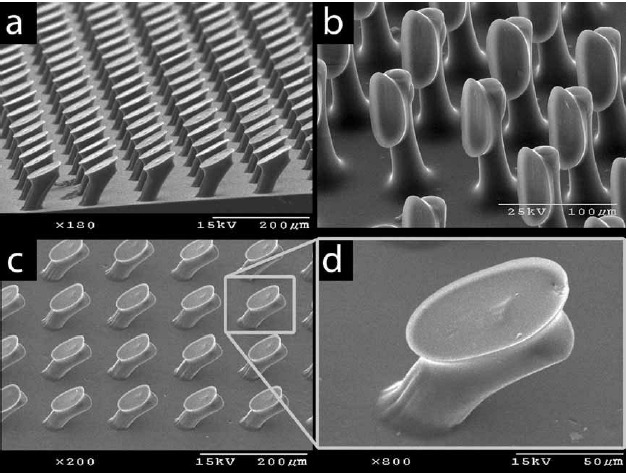
\includegraphics[width=0.70\textwidth]{Gecko1}
	\caption{Aufnahme einer Mikrostruktur mit 35 $\mu m$ Durchmesser. Strukturen weisen unterschiedliche Winkel auf: a) 	34\textdegree{}  b) 90\textdegree{}  c/d) 23\textdegree{} \cite{Schwerter.}}
	\label{fig:Gecko1}
\end{figure}


Bei der technischen Anwendung ist zu beachten, dass es eine Haftrichtung und eine Ablöserichtung in der Struktur gibt. Die haltbaren Scherkräfte in Ablöserichtung sind somit um bis zu Faktor zehn geringer als in Haftrichtung \cite{Schwerter.}.
In der Simulation (\abb{fig:Gecko2}) ist gut zu erkennen, dass die Mikrosäulen mit dem Haftprofil in eine vorbestimmte Richtung belastet werden sollen. Andernfalls können sie nicht die maximale Haftfläche nutzen und es geht Haftkraft verloren \cite{Schwerter.}. 


\begin{figure}[H]
	\centering
		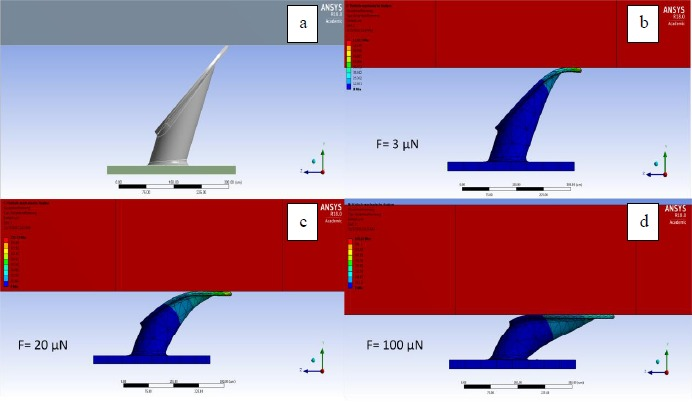
\includegraphics[width=0.70\textwidth]{Gecko2}
	\caption{Simulation des Verformungsverhaltens der Mikrostruktur bei Haftberührung \cite[Abbildung 19, Seite43]{Schwerter.}}
	\label{fig:Gecko2}
\end{figure}	


Allgemein wird eine Steigerung der Normalkraft und der Scherkräfte durch Erhöhung der Anpresskraft festgestellt. Optimaler Halt sollte also mit einer Vorspannkraft, die beim anbringen der Mikrostruktur ausgeübt wird erreicht werden \cite{Schwerter.}. Die genaue Funktion und die entstehenden Kräfte sind bei den verschiedenen Geometrien und eingesetzten Materialien unterschiedlich. Eine genaue Auflistung der erreichten Haftkräfte für die verschiedenen Ausführungen der Mikrostruktur und Belastungsfälle ist in \cite[Tabelle 1]{Schwerter.} zu finden.

Polydimethylsiloxan (PDMS) Strukturen erreichen maximale Scherkräfte in Haftrichtung von \SI{34,8}{\newton\per\square\milli\metre} und einer Normalkraft von \SI{10,8}{\newton\per\square\milli\metre}.
Es wurde durch mehrere Versuchsreihen nachgewiesen, dass Temperatur und Vakuum kaum einen Einfluss auf die Leistungsdaten haben. Verschiedene Mikrostrukturen wurden einer thermischen Wechselbeanspruchung zwischen 125 und -125 \textdegree{} C unterzogen und daraufhin in Vakuum und Normalbedingungen getestet. Durch die Temperatur ist kein Einfluss zu verzeichnen. Das Vakuum ruft nur vernachlässigbare Änderungen in Vorspannung und Haftung hervor \cite[Bild 11]{Trentlage.}. Durch Tests mit verschiedenen Materialien konnte festgestellt werden, dass die Oberfläche, an der die Struktur haften soll einen relativ geringen Einfluss auf die Haftung hat \cite[Bild 16]{Trentlage.}.


Gecko-inspirierte Mikrostrukturoberflächen scheinen eine vielversprechende Lösung für das Dockingproblem bei ADR Missionen zu sein. Für das Docking muss etwas genutzt werden, das den Bedingungen im Weltraum wie Vakuum, Strahlung und Kälte standhält. Besonders vorteilhaft ist das zerstörungsfreie Andocken mittels der Geckostruktur, was das Risiko neu entstehender Trümmerteile verringert. Für diese Anwendung sollen Geckomaterialien näher untersucht werden. Es existiert bereits ein Andockmechanismus (\abb{fig:Gecko3}) dessen Gecko-Mikrostruktur nach  European Cooperation for Space Standardization (ECSS) Standards getestet wurde \cite[Seite 10]{ChristopherTrentlage.2018}. Durch einen Versteifungsmodus und die aktive Lastverteilung wird eine möglichst gute Verteilung der herrschenden Kräfte erzielt \cite{ChristopherTrentlage.2018}. Außerdem wurden PDMS Strukturen bereits erfolgreich in der Schwerelosigkeit getestet. Diese konnten an einem Greifer verschiedene Objekte einfangen und bewegen \cite{Schwerter.}.



\begin{figure}[H]
	\centering
		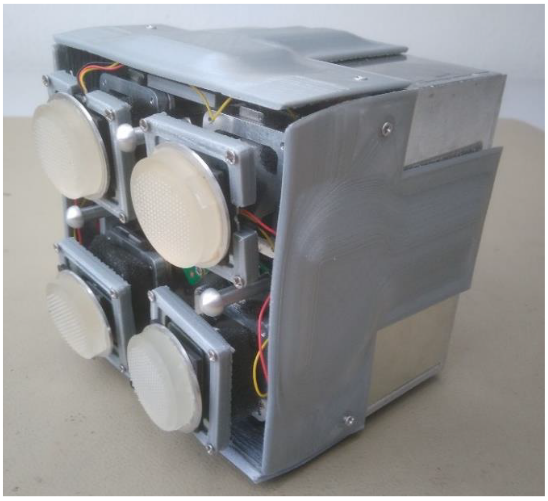
\includegraphics[width=0.50\textwidth]{graphics/Gecko3.PNG}
	\caption{Prototyp Gecko Dochingmechanismus \cite[Figure 18, Seite 10]{Trentlage.}}
	\label{fig:Gecko3}
\end{figure}



Für die folgende Abschätzung der maximal wirkenden Kräfte auf die Mikrohaftstruktur wurde der Aufbau des Prototypen (\abb{fig:Gecko_Rechnung1}) vorausgesetzt. Bei den Berechnungen wird von den ungünstigsten Lastfällen ausgegangen.
In den Abbildungen \ref{fig:Gecko_Rechnung1}, \ref{fig:Gecko_Rechnung2} und \ref{fig:Gecko_Rechnung3} werden die der Berechnung zugrundeliegenden Annahmen gezeigt. Die belasteten Verbindungen der Mikrohaftstrukturen zum Zielobjekt werden als feste Lager A und B angenommen. Es wird davon ausgegangen, dass die Vorspannkraft beim Andocken ideal aufgebracht wurde. Außerdem bleibt die Kombination aus kritischen Normal- und Scherkräften unberücksichtigt. Der zusätzliche Anpressdruck des Haupttriebwerks wurde ebenfalls nicht berücksichtigt.

\begin{figure}[H]
	\centering
		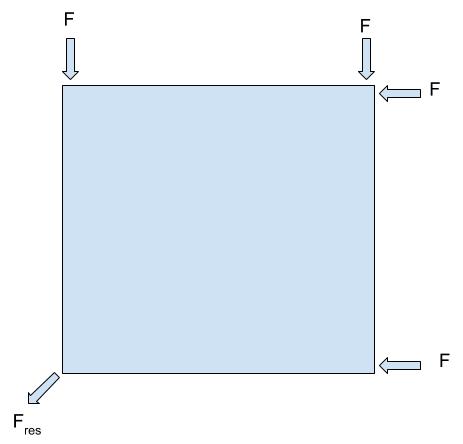
\includegraphics[width=0.50\textwidth]{graphics/Gecko_Rechnung1.png}
	\caption{Kräftebetrachtung Ansicht von oben}
	\label{fig:Gecko_Rechnung1}
\end{figure}

\begin{figure}[H]
	\centering
		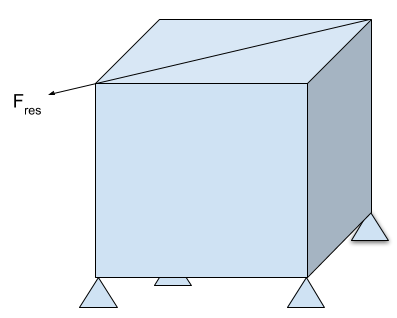
\includegraphics[width=0.50\textwidth]{graphics/Gecko_Rechnung2.png}
	\caption{Kräftebetrachtung 3D}
	\label{fig:Gecko_Rechnung2}
\end{figure}

\begin{figure}[H]
	\centering
		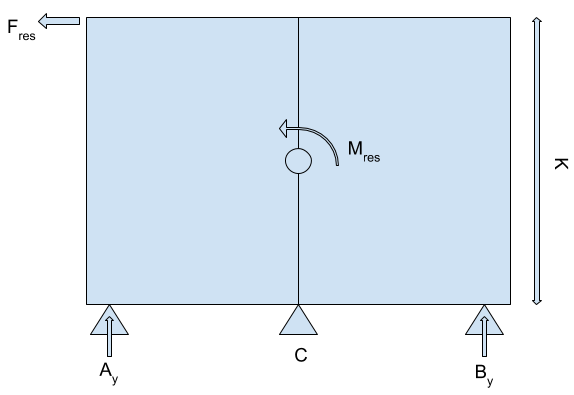
\includegraphics[width=0.50\textwidth]{graphics/Gecko_Rechnung3.png}
	\caption{Kräftebetrachtung Momentengleichgewicht}
	\label{fig:Gecko_Rechnung3}
\end{figure}


	Wie in \abb{fig:Gecko_Rechnung1} und \abb{fig:Gecko_Rechnung2} zu erkennen ist wirken bei der maximalen Belastung durch Normalspannung vier Düsen des RCS-Systems mit einem Schub von jeweils \SI{0,23}{\newton} \kap{cap:AngenommenesDesign}. Die auftretenden Kräfte werden zur resultierenden Kraft $F_{res}$  zusammengefasst:

	\begin{eqnarray}
			F_{res}=\sqrt{ 2 }*2F
	\end{eqnarray}

	Über das Momentengleichgewicht lässt sich die wirkende Kraft in y-Richtung des Festlagers $B_y$  bestimmen (\abb{fig:Gecko_Rechnung3}).

\begin{eqnarray}
		\sum{  }{  }{ M_{(C)} }=0=-B_y*CB+AC*A_y+F_{res}*K
\end{eqnarray}
	$B_y$ entspricht der maximalen Normalkraft, die einen Haftpunkt belasten kann. Mit einer Sicherheit von \num{5} ergibt sich eine maximale Normalkraft $N_{max}$ von \SI{3,25}{\newton}. Um die maximal auftretende Scherkraft zu bestimmen wird der Schub von allen vier RCS-Triebwerken einer Seite angenommen. Demzufolge ergibt sich mit einer Sicherheit $S = 5$ eine maximale Scherkraft von $F_{S, max} =$ \SI{4,6}{\newton}, die sich auf jeden der vier Haftpunkte verteilt. Zur Berechnung der nötigen Fläche der Mikrohaftstruktur werden die Werte für PDMS Material mit Säulengeometrie aus \cite[Tabelle1, Seite 23]{Schwerter.} verwendet. Die Dimensionierung wird über $N_{max}$ des Belastungsfalles bestimmt. Da diese Kraft einen einzelnen Haftfuß belastet, ist sie ausschlaggebend zur Dimensionierung. Es ergibt sich mit einer Gesamtsicherheit von \num{5} eine minimale Haftfläche von \SI{4,9}{\centi\metre\squared} für jeden Haftpunkt. Der ermittelte Wert beruht auf der Annahme einer ideal aufgebrachten Vorspannkraft durch das Andocken. Durch die Berücksichtigung der Sicherheit sollten alle zuvor bestimmten Annahmen ausreichend ausgeglichen werden. 




		
						%\textbf{Was sind Geckomaterialen}
						%\textbf{Bisher getestete Gecko-Materialien}
						%\textbf{Bisherige Erfolge}
						%\textbf{State of the Art}
						%\textbf{Problematik}